\chapter{Appendix} \label{chapter: Appendix}

\begin{code}[htpb]
    \centering
    \begin{tabular}{c}
    \begin{lstlisting}[language=ruby]
apiVersion: apps/v1
kind: DaemonSet
metadata:
    name: green-daemon
    namespace: default
spec:
    selector:
        matchLabels:
            name: green-daemon
    template:
        metadata:
            labels:
                name: green-daemon
        spec:
            containers:
            - name: green
              image: led-daemon
              args:
              - GREEN
            nodeSelector:
                type: "virtual-kubelet"
                model: "raspberry-pi"
                light: "GREEN"
            tolerations:
            - key: "virtual-kubelet.io/provider"
              operator: "Equal"
              value: "unikernel"
              effect: "NoSchedule"
  \end{lstlisting}
  \end{tabular}
  \caption{Green-daemon specification}\label{fig:green-daemon}
  \end{code}


\begin{code}[htpb]
    \centering
    \begin{tabular}{c}
    \begin{lstlisting}[language=ruby]
apiVersion: apps/v1
kind: Deployment
metadata:
    name: humidity
    labels:
        app: humidity
spec:
    selector:
        matchLabels:
            app: humidity
    template:
        metadata:
            labels:
                app: humidity
        spec:
            containers:
            - name: unikernel
              image : sensor.native
              env:
              - name: "sensor"
                value: "humidity"
            nodeSelector:
                type: "virtual-kubelet"
                model: "raspberry-pi"
            tolerations:
            - key: "virtual-kubelet.io/provider"
              operator: "Equal"
              value: "unikernel"
              effect: "NoSchedule"
\end{lstlisting}
\end{tabular}
\caption{Unikernel specific deployment}\label{fig:unikernel-dep}
\end{code}


\begin{code}[htpb]
    \centering
    \begin{tabular}{c}
    \begin{lstlisting}[language=ruby]
from kubernetes import client, config,watch

def isUnreachable(t):
        return t.effect=="NoSchedule" and t.key=="node.kubernetes.io/unreachable"
        
def main():
    config.load_incluster_config()
    api=client.CoreV1Api()
    
    w=watch.Watch()
    for change in w.stream(api.list_node,timeout_seconds=0):
        node=change["object"]
        if change["type"]=="MODIFIED": # from ready to not ready
            try:
                for t in node.spec.taints:
                    if isUnreachable(t):
                        api.delete_node(node.metadata.name)
                        print("Deleting node because it's not reachable")
            except TypeError:
                print("No taints")

if __name__=="__main__":
    main()

\end{lstlisting}
\end{tabular}
\caption{NodeWatcher code}\label{fig:nodewatcher}
\end{code}

\begin{code}[htpb]
    \centering
    \begin{tabular}{c}
    \begin{lstlisting}[language=caml,showstringspaces=false,breaklines=true,upquote=true]
        open Lwt.Infix

        module Main (KV: Mirage_kv.RO) (Time: Mirage_time.S) = struct
        
          let start kv _time=
        
            let read_from_file kv filename = (*Filename given as argument*)
                KV.get kv (Mirage_kv.Key.v filename) >|= function
                    | Error e ->
                        Logs.warn (fun f -> f "Cannot find the file %a"
                        KV.pp_error e)
                    | Ok sensor_value ->
                        Logs.info (fun f -> f "Reading from: %s -> %s" filename sensor_value);
            in
                let filename=Key_gen.filename() in
                let rec loop() =
                read_from_file kv filename >>= fun()->
                Time.sleep_ns (Duration.of_sec 2)>>= fun () ->
                loop()
                in 
                loop()
        end
  \end{lstlisting}
  \end{tabular}
  \caption{A MirageOS program}\label{fig:ocaml-demo}
\end{code}


\iffalse
  \begin{figure}
    \centering
    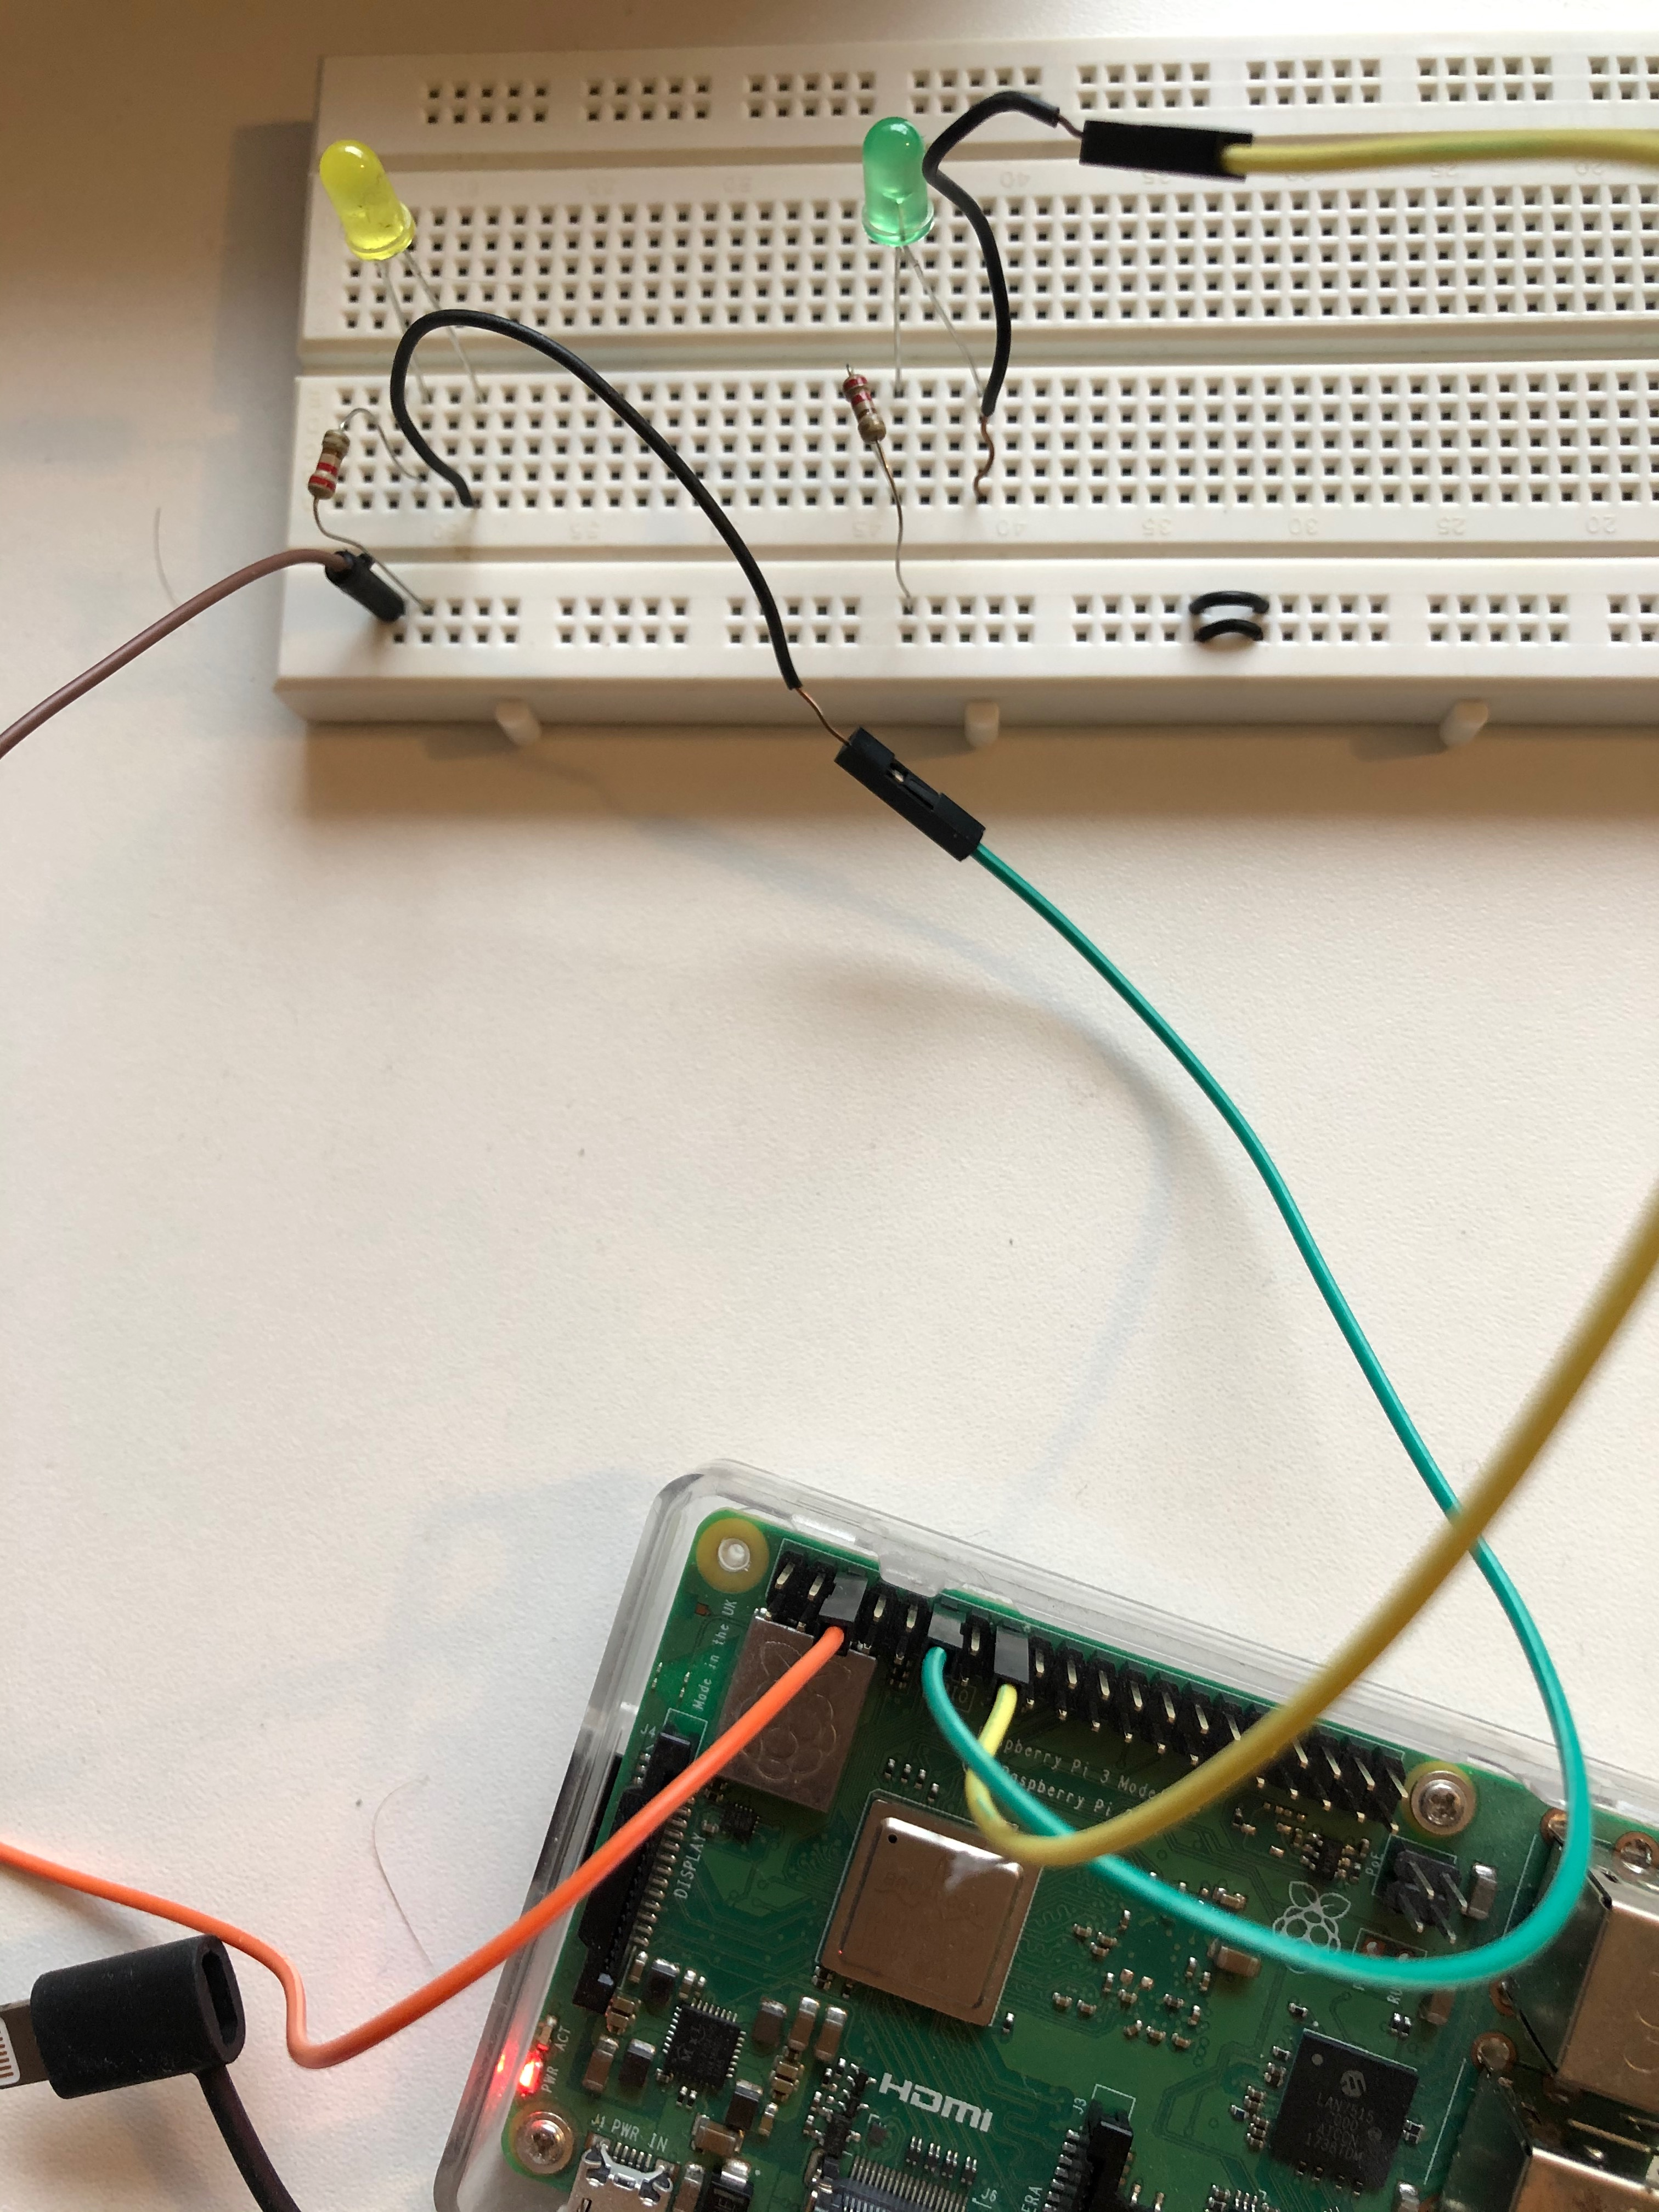
\includegraphics[width=0.9\textwidth]{rasp-running.jpeg}
    \caption{Photo of wiring of \ref{fig:rpi-diagram}}\label{fig:wiring}
  \end{figure}
\fi